\documentclass[aspectratio=169, t, 10pt,
%    ignorenonframetext,
    ]{beamer}
\usetheme{Boadilla}
\beamertemplatenavigationsymbolsempty

\usepackage{standalone}
\usepackage[utf8]{inputenc}
\usepackage[english]{babel}
\usepackage{pgfplots}
    \usetikzlibrary{shapes, positioning}
\usepackage{mathtools}
\mathtoolsset{showonlyrefs}
\usepackage{qrcode}
\usepackage{multimedia}

\newcommand\Mean[1]{\mathbb{E}\!\left[#1\right]}
\newcommand\Var[1]{\mathbb{V}\!\left[#1\right]}
\newcommand\Cov[2]{\mathrm{Cov}\!\left[#1,#2\right]}
\newcommand\Gauss[2]{\mathcal{N}\!\left({#1},\,{#2}\right)}
\newcommand\GP[2]{\mathcal{GP}\!\left({#1},\,{#2}\right)}
\newcommand{\Identity}{\mathbb{I}}

\title[Correlation based travel time inversion]{Bayesian Travel Time Inversion adopting Gaussian Process Regression}
\subtitle{-- with a focus on uncertainty analysis --}
\author[\tt mauerber@uni-potsdam.de]{Stefan Mauerberger \and Matthias Holschneider}
\institute[Math@UP]{University Potsdam, Institute of Mathematics}
\titlegraphic{%\vspace{-1cm}
              \hspace{2cm}
              \parbox[c]{0.17\linewidth}{
\includegraphics[width=\linewidth]{./logos/GeoSim_Logo}}
              \hfill
              \parbox[c]{0.10\linewidth}{
\includegraphics[width=\linewidth]{./logos/UniPotsdam_Logo}}
              \hspace{2cm}
              }
\date[AGU~2017]{AGU Fall Meeting -- 13\textsuperscript{th} December 2017}

\input{def_example}
\begin{document}

\frame[noframenumbering, plain]
    {\maketitle}

Looking into the Earth is one of the major applications in seismology.
\\
I am going to provide new insight into travel time inversion from a statistical point of view.


\begin{frame}
    \frametitle{Seismic Tomography}
    \framesubtitle{~}%
%
\begin{columns}%
\column{.55\textwidth}%
%
    \begin{itemize}
        \item Credibility increase of the model?
        \item Statistical significance of structures?
    \end{itemize}

    \begin{center}
        \large Uncertainties are required to evaluate the model
    \end{center}

    \begin{exampleblock}{New approach in Travel Time Inversion}
    \begin{itemize}
        \item Bayesian inversion
        \item Correlation based
        \item Non-parametric
        \item Computationally inoffensive
    \end{itemize}
    \hfill {\large$\leadsto$} Posterior distribution ~
    \end{exampleblock}

\column[T]{.44\textwidth}
    \vspace{-10mm}
    \input{fig_realization_pst.pgf}
\end{columns}

\end{frame}


Although seismic tomography has widespread applications, credibility is one of the pressing questions.
\\
As an example, are those structures of statistical significant or is this just a random realization?
\\[2mm]

Putting seismic tomography into a rigorous statistical setting may answer that question.
\\
To assess uncertainties I am going to introduce a new Bayesian method in travel time inversion.
\\
The posterior velocity model is derived using a correlation-based and non-parametric approach at ordinary computational costs.


\begin{frame}
    \frametitle{Synthetic Test}
    \framesubtitle{proof of concept}%
%
\begin{columns}%
\column{.55\textwidth}%
%

    \begin{exampleblock}{Setting}
        \begin{itemize}
            \item Large scale anomalies as a reference model
            \item Neglecting dispersion and refraction
            \item Station geometry borrowed from ScanArray
        \end{itemize}
    \end{exampleblock}
    \medskip

    \begin{alertblock}{Infer reference model from travel time obs.}
        Bayesian posterior distribution \\
        \hfill {\large $\leadsto$} Location dependent model uncertainties ~
    \end{alertblock}

\column[T]{.44\textwidth}
    \vspace{-10mm}
    \input{fig_reference_model.pgf}
\end{columns}

\end{frame}

As a demonstration, a subset of $\SFWnst$ stations of the ScanArray is considered.
\\
The reference model is composed of two large scale anomalies; approximately 4\% peak to peak.
\\
Travel times are generated from that model neglecting refraction and dispersion.
\\
The aim of the example is to recover the reference model posterior to travel time data.
\\
Again, it is the model's uncertainty which is of particular interest.


\begin{frame}
    \frametitle{Travel Time Observations}
    \framesubtitle{a non-linear functional w.r.t.~the velocity model}

\begin{columns}
\column{.55\textwidth}%
    \begin{equation}
        \mathrm T_C[v] = \int_C \frac 1{v(r)} \mathrm d r
    \end{equation}

    \begin{description}[leftmargin=! ,labelwidth=1cm]
        \item [Observational functional] $\mathrm T_C[\,\cdot\,]$
        \item [Ray path]                 $C_{s,r}[\,\cdot\,]$
        \item [Source location]          $s$
        \item [Receiver position]        $r$
        \item [Velocity model]           $v$
    \end{description}

    \begin{alertblock}{It is the velocity model what we are after}
    \begin{itemize}
        \item Travel times are putting an Integral-constraint on $v$
        \item Non-linearity is a major concern
    \end{itemize}
    \end{alertblock}


\column[T]{.44\textwidth}
    \vspace{-10mm}
    \only{\input{fig_path_coverage.pgf}}
    \small
    \begin{align}
        N_\text{stn} &= \SFWnst &
        & \leadsto &
        N_\text{obs} &= \SFWnobs
    \end{align}

\end{columns}

\end{frame}

Travel times are expressed in terms of an integral over the slowness along the ray path.
\\
The observational functional is putting an integral constraint on the velocity model.
\\
However, the non-linear relation of travel times and velocity model is a challenge.
\\[2mm]

In the example, travel times are calculated for all station pairs.
\\
The resulting $\SFWnobs$ records are corrupted by normal noise.
\\[2mm]

Before going ahead with non-linearity lets have a look at the a\,priori assumptions.


\begin{frame}
    \frametitle{A\,Priori Velocity Model}
    \framesubtitle{expressing our ignorance}

\begin{columns}
\column{.55\textwidth}%
    \begin{block}{Assume the model a Gaussian Random Field}
    \begin{equation}
        v \to V \sim \GP{\mu_V}{K_V}
    \end{equation}
    \begin{description}[leftmargin=! ,labelwidth=6cm]
        \item [Prior mean function] $\mu_V(x) = \SFWmuCpri \, \frac ms$
        \item [Covariance function] $K_V(x,y)$
    \end{description}
    \end{block}
    \medskip

    Assumed covariance
    \begin{equation}
        K_V(x,y) = \tau^2 \exp\left\{ -\frac12 \frac{d(x,y)^2}{\ell^2}\right\}
    \end{equation}
    \begin{description}[leftmargin=! ,labelwidth=6cm]
        \item [Great circle distance] $d(x,y)$
        \item [Standard deviation]   $\tau = \SFWtau \, \frac ms$
        \item [Characteristic length]  $\ell = \SFWell \, m$
    \end{description}

\column[T]{.44\textwidth}
    \centering
    \vspace{-10mm}
    \input{fig_kernel_pri.pgf}

\end{columns}

\end{frame}

To express our ignorance, the a\,priori velocity model is assumed a Gaussian random field.
\\
It is fully determined by its mean function and covariance function.
\\[2mm]

For the example, I basically use a constant mean of $\SFWmuCpri \, \frac ms$.
\\
A spherical distance based squared exponential kernel is assumed.
\\
The characteristic length is $\SFWell \, m$ and the deviation from the mean is $\SFWtau \, \frac ms$.
\\[2mm]

The kernel is depicted on the right.
\\
The further two points are apart the less correlated they are.
\\
In turn, close by points are likely to share similar velocities.


\begin{frame}
    \frametitle{Linearization}
    \framesubtitle{Gaussianity is preserved under linear maps}

\begin{columns}
\column{.55\textwidth}%
    \begin{equation}
        \mathrm T_C[V] \approx \int_C \frac 1{\mu_V(r)} - \frac{V(r)}{\mu_V(r)^2} \, \mathrm d r
    \end{equation}
    \begin{description}[leftmargin=!, labelwidth=1cm]
        \item [Taylor expansion] 1\textsuperscript{st} order
        \item [point of expansion] $\mu_V$ (prior mean)
    \end{description}
    \medskip

    \begin{block}{Approximated correlation}
    \begin{equation}
        \Cov{V}{\mathrm T_C[V]\,} \approx -\int_C \frac {K_V(\cdot,r)}{\mu_V(r)^2} \, \mathrm d r
    \end{equation}
    \end{block}

    \begin{block}{Approximated co-variance}
    \setlength\abovedisplayskip{0pt}
    \begin{equation}
        \Cov{\mathrm T_C[V]}{\mathrm T_{C'}[V]\,} \approx  \int_C \int_{C'} \frac{K_V(r,r')}{\mu_V(r)^2\mu_V(r')^2} \, \mathrm d r \, \mathrm d r'
    \end{equation}
    \end{block}

\column[T]{.44\textwidth}
    \centering
    \vspace{-10mm}
    \input{fig_correlation_pri.pgf}
    \\ \scriptsize
    Prior correlation of $V(x)$ with $T_C[V]$ kept fix

\end{columns}

\end{frame}

In case of non-linearities, it is not feasible to compute the full Bayesian posterior.
\\
Therefore, we are looking only at first order fluctuations.
\\
A Taylor expansion around the prior mean function turns correlations and co-variances into explicit formulas.
\\
The line integrals are solved numerically.
\\[2mm]

The figure on the right shows the prior correlation of an observation and the model.
\\
It illustrates what is learned about the medium from a single measurement.



\begin{frame}
    \frametitle{Bayesian Posterior Distribution}
    \framesubtitle{Gaussian Process Regression}

\begin{columns}
\column[t]{.55\textwidth}

    \vspace{-1mm}
    \begin{description}[labelwidth=25mm]
        \item [Prior travel times] $\mu_D = \Mean{\mathrm T_C[\mu_V]\,}$
        \item [Covariance matrix]  $\Sigma_{DD} = \Cov{\mathrm T_C}{\mathrm T_{C'}} + \Identity \sigma_\varepsilon^2$
    \end{description}
    \vspace{-1mm}

    \begin{exampleblock}{Conditional mean and covariance}
        \setlength\abovedisplayskip{0pt}
        \begin{alignat}{3}
            \Mean{V|d} &= \mu_V &&+ \Cov VD \Sigma_{DD}^{-1} \big( d - \mu_{D} \big)
            \\
            \Var{V|d}  &= K_V   &&- \Cov VD \Sigma_{DD}^{-1} \Cov DV
        \end{alignat}
        \hfill $\leadsto$ Posterior distribution ~
    \end{exampleblock}

    \begin{alertblock}{Accommodate non-linearity}
        \begin{itemize}
            \item Single evidence at a time
            \item Correlations and Variances from predecessor
        \end{itemize}
        \hfill  $\leadsto$ Successive approach ~
    \end{alertblock}

\column[T]{.44\textwidth}
    \vspace{-5mm} \centering
    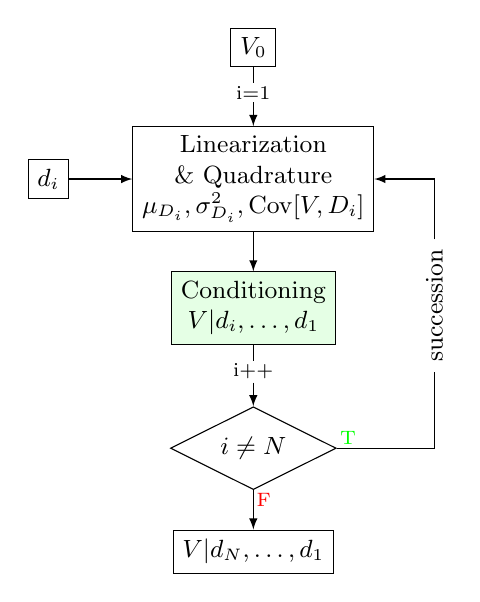
\begin{tikzpicture}[font=\small]
        \tikzstyle{decision} = [diamond, draw, aspect=2]
        \tikzstyle{block} = [rectangle, draw, align=center]
        \tikzstyle{line} = [-latex]
        \node (pri) [block] {$V_0$};
        \node [below=2mm of pri] (int) [inner sep=1pt] {\scriptsize i=1};
        \node [below=3mm of int] (lin) [block] {Linearization \\ \& Quadrature\\ $\mu_{D_i}, \sigma_{D_i}^2, \Cov V{D_i}$};
        \node [left=8mm of lin]  (dat) [block] {$d_i$};
        \node [below=5mm of lin] (cnd) [block, fill=green!10] {Conditioning \\ $V|d_i,\dots,d_1$};
        \node [below=2mm of cnd] (inc) [inner sep=1pt] {\scriptsize i++};
        \node [right=2cm of inc] (suc) [rotate=90] {succession};
        \node [below=3mm of inc] (dec) [decision] {$i\neq N$};
        \node [below=5mm of dec] (pst) [block] {$V|d_N,\dots,d_1$};
        \node at (dec.east)  [anchor=south west, inner sep=1pt, green] {\scriptsize T};
        \node at (dec.south) [anchor=north west, inner sep=1pt, red] {\scriptsize F};

        \draw [line] (dat) -- (lin);
        \draw [line] (lin) -- (cnd);
        \draw [line] (dec) -| (suc) |- (lin);
        \draw [line] (pri) -- (int) -- (lin);
        \draw [line] (cnd) -- (inc) -- (dec);
        \draw [line] (dec) -- (pst);
    \end{tikzpicture}



\end{columns}

\end{frame}

A data model accounting for normal noise is chosen.
\\
Travel times are assumed being accurate at about $\SFWepsilon\,s$.
\\[2mm]

The posterior distribution is given by conditional mean and covariance.
\\
This is a non-parametric model in the sense considering a distribution over functions.
\\
Neither coefficients nor basis functions are involved.
\\
The kernel spans a function space and the conditional is rating down functions incompatible with data.
\\[2mm]

To accommodate non-linearity I pursue a successive strategy similar to a Kalman filter.
\\
At each step only a single evidence is incorporated.
\\
The linearization and conditioning are performed again and again till the last evidence is caught.
\\
While progressing, the posterior mean improves gradually.
\\
The closer the point of expansion to reality the better the Taylor expansion performs.


\begin{frame}
    \frametitle{Successive Approach}
    \begin{center}
    \movie[height=0.85\textheight, width=1.51\textheight, autostart]{\includegraphics[height=0.85\textheight, width=1.51\textheight]{animation_pst}}{animation.avi}
    \end{center}
\end{frame}

To illustrate the idea, I prepared a little video.
\\
The left hand panel shows how the conditional mean develops.
\\
Contour lines are for comparison with the reference model.
\\
On the right, the evolution of the conditional standard deviation is depicted.
\\[2mm]

The path by path construction can nicely be seen.
\\
Both anomalies are captured.
\\
The characteristic length is reflected by the extent of the patches.
\\
Areas of dense ray coverage are showing highest confidence gain.
\\
\pgfmathparse{int(round(\SFWsdred/\SFWtau*100))}
The variance reduction is $\pgfmathresult$\%.

\begin{frame}
    \frametitle{Results}
    \framesubtitle{~}

\begin{columns}
\column{.55\textwidth}%

    \begin{itemize}
        \item Anomalies caught
        \item Spatial uncertainty
        \item Variance reduction $\Delta\sigma = \SFWsdred$
    \end{itemize}

    \begin{itemize}
        \item Analogy with sensitivity kernels
        \item Increase in complexity
        \item Small scale correlations
        \item Reduction correlation
        \item Anti correlation
    \end{itemize}


\column[T]{.44\textwidth}
    \vspace{-10mm}
    \centering \scriptsize
    \only<1>{\input{fig_correlation_pst.pgf} \\
    Posterior correlation of $V(x)$ with $T_C[V]$ kept fix }
    \only<2>{\input{fig_correlation_pri.pgf}\\
    ~~ Prior correlation of $V(x)$ with $T_C[V]$ kept fix }
\end{columns}

\end{frame}

Correlation of a single travel time measurement with the model posterior to observations.
\\


\begin{frame}
    \frametitle{Conclusions}
    \framesubtitle{Assessment of Uncertainties}

\begin{columns}
\column{.55\textwidth}%

    \begin{exampleblock}{Bayesian Posterior Distribution}
    \begin{itemize}
        \item Posterior Covariance \hfill $\leadsto$ \hfill Uncertainties
        \item Succession \hfill $\leadsto$ \hfill Accommodates non-linearity
        \item Function space view \hfill $\leadsto$ \hfill Non-Parametric
    \end{itemize}
    \end{exampleblock}


\column[T]{.44\textwidth}
    \vspace{-10mm}
    \centering
    \only{\documentclass[beamer=true]{standalone}
\usepackage{pgfplots}
\input{def_example}
%
\begin{document}
\begin{tikzpicture}
    \pgfplotstableread{./dat/misfit.dat}\misfit
    \pgfplotsset{axis lines=left, tick label style={font=\tiny}, log ticks with fixed point}
    \begin{semilogyaxis}[width=\textwidth, height=\textheight,
             ylabel={Data misfit}, xlabel={\# evidence}, ylabel near ticks,
             legend cell align=left,  xlabel near ticks,
             legend style={only marks, draw=none, font=\footnotesize,
             at={(0,0)}, anchor=south west },
             label style={font=\scriptsize}, name=big ]
        \addplot [dashed, mark=*, blue , mark options={scale=0.5, solid}] table [x=evd, y=all] \misfit;
        \addlegendentry{all at once}
        \addplot [dashed, mark=*, red  , mark options={scale=0.5, solid}] table [x=evd, y=asc] \misfit;
        \addlegendentry{ascending $\sphericalangle$}
        \addplot [dashed, mark=*, green, mark options={scale=0.5, solid}] table [x=evd, y=dsc] \misfit;
        \addlegendentry{descending $\sphericalangle$}
        \addplot [dashed, mark=*, black, mark options={scale=0.5, solid}] table [x=evd, y=rnd1] \misfit;
        \addlegendentry{shuffle}
        \addplot [dashed, mark=*, black, mark options={scale=0.5, solid}] table [x=evd, y=rnd2] \misfit;
    \end{semilogyaxis}
    \begin{axis}[at=(big.north east), anchor=north east, width=0.5\textwidth, height=0.5\textwidth,
                 xmin={\SFWnobs-14}, xmax={\SFWnobs+3}]
        \addplot [dashed, mark=*, red  , mark options={scale=0.5, solid}] table [x=evd, y=asc] \misfit;
        \addplot [dashed, mark=*, green, mark options={scale=0.5, solid}] table [x=evd, y=dsc] \misfit;
        \addplot [dashed, mark=*, black, mark options={scale=0.5, solid}] table [x=evd, y=rnd1] \misfit;
        \addplot [dashed, mark=*, black, mark options={scale=0.5, solid}] table [x=evd, y=rnd2] \misfit;
    \end{axis}
\end{tikzpicture}
\end{document}

}
\end{columns}

\end{frame}

Data misfit
succession outperforms all-at-once
Resolution is not limited by a certain parametrization.


\begin{frame}
    \frametitle{Outlook \& Next Steps }
    \framesubtitle{Potential future application}

\begin{columns}
\column{.55\textwidth}%

    \begin{itemize}
        \item Poisson type kernel
        \item Estimation of hyper parameters
        \item Adaptive grid to facilitate refraction
    \end{itemize}

    \begin{block}{Surface Wave Tomography}
        \begin{itemize}
            \item Model phase velocities $v(\omega)$
            \item Use ambient noise records
            \item Frequency-space dependent kernel
                \begin{equation}
                    K(x,\omega; x', \omega')
                \end{equation}
                accounting for dispersion
        \end{itemize}
    \end{block}

\column[T]{.44\textwidth}
    \centering
    \only<1>{\vspace{-12mm}
        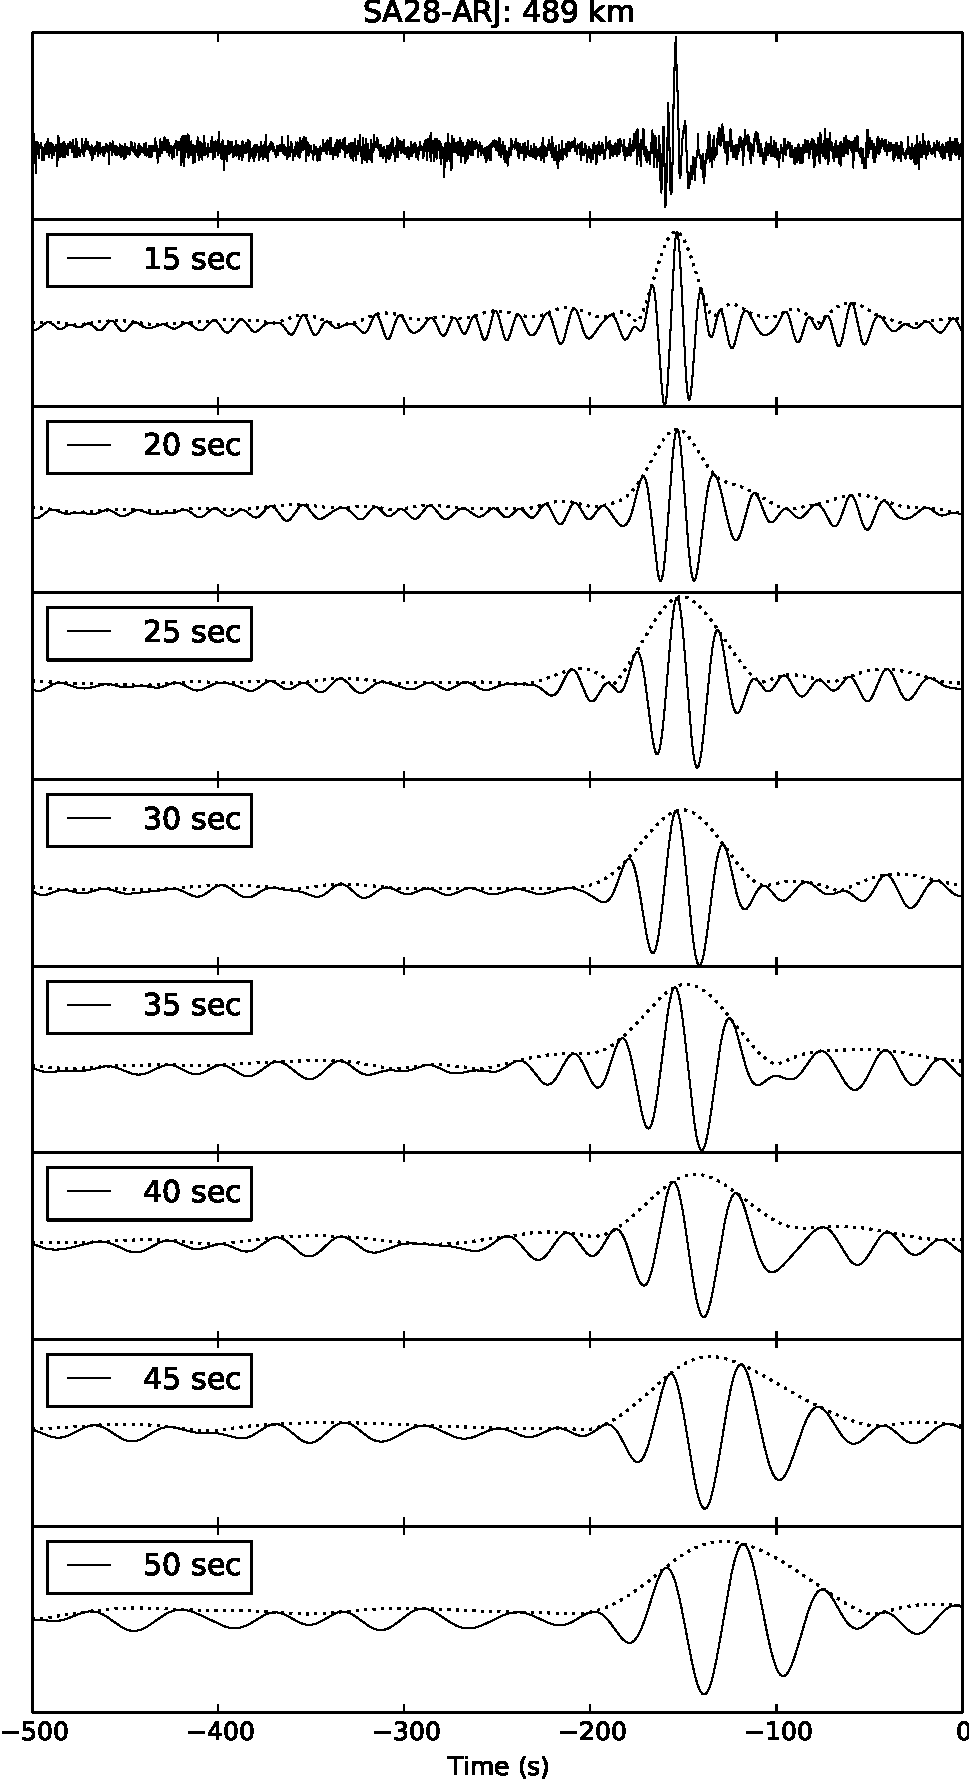
\includegraphics[height=0.9\textheight]{MultiFiltered_SA28-ARJ}
        \\
        \tiny Multi-filtered correlogram by courtesy of A.~Mauerberger
    }
    %\only<2>{
    %    \vspace{2mm}
    %    Follow the project on GitHub
    %    \\[6mm]
    %    \fbox{\qrcode[height=3cm]{https://github.com/mauimuc/gptt}}
    %    \\[6mm]
    %    \small
    %    \href{https://github.com/mauimuc/gptt}{github.com/mauimuc/gptt}
    %}
\end{columns}

\end{frame}

For spherical geometries the usage of a Poisson type kernel is natural.
\\
A maximum likelihood estimate appears adequate to guess prior mean and error level.
\\
However, a clever strategy is necessary estimting the characteristic length.
\\
Implement refraction and
adjust discretization for changes in the ray path.
\\[2mm]

Modeling phase velocities is a potential future application.
\\
Surface waves are showing strong dispersion, clearly visible in the correlogram on the right.
\\
To model phase velocities a frequency dependent kernel is required.
\\
A simple departure is a locally stationary kernel.
\\
Both characteristic length and variance are assumed to depend on the centroid and/or lag frequency.
\\[2mm]

Thanks for your attention; Looking forward to your questions.

\end{document}
